
\documentclass{article}

%% Packages for French writing
\usepackage[french]{babel}
\usepackage[utf8]{inputenc}
\usepackage[T1]{fontenc}
\usepackage{layout}

%% Packages for Math symbols
\usepackage[fleqn]{amsmath}
\usepackage{amssymb}
\usepackage{mathrsfs}

%% Packages for figures insertion
\usepackage{graphicx}
\usepackage{wrapfig}
\usepackage{framed}
\usepackage{float}

%% Package for document margin editing
\usepackage[top=2cm, bottom=2cm, left=2cm, right=2cm]{geometry}

%% Package for source code insertion
\usepackage{listings}
\usepackage{xcolor}
\definecolor{grey}{rgb}{0.97, 0.97, 0.97}
\definecolor{darkred}{rgb}{0.42, 0, 0}
\definecolor{darkblue}{rgb}{0, 0, 0.42}
\definecolor{darkgrey}{rgb}{0.22, 0.22, 0.82}
\definecolor{green}{HTML}{088A08}
\lstset{
  basicstyle=\small\sffamily\footnotesize,
  captionpos=b,
  numbers=left,
  numberstyle=\tiny,
  tabsize=4,
  frame=trBL,
  backgroundcolor=\color{grey},
  commentstyle=\color{green},
  keywordstyle=\color{darkblue}\bf,
  identifierstyle=\color{darkgrey},
  stringstyle=\color{darkred}
}

\setlength\parindent{0pt}
\setlength\parskip{3pt}
\title{ARCHI2 - Compte-rendu du TME2}
\author{Nicolas Phan}
\date{pour le 23 Février 2018}
\begin{document}
\pagestyle{headings}
\maketitle
\tableofcontents
\newpage

%===============================================================================
%=========================  Introduction  ======================================
%===============================================================================


\section{Automate du composant PibusSimpleRam}

\begin{figure}[H]
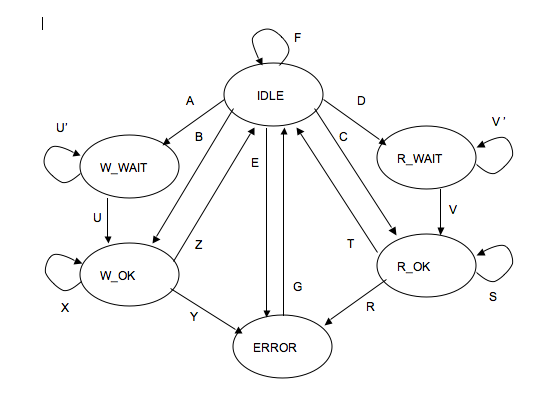
\includegraphics[width=0.75\textwidth]{pics/mae_ram.png}
\centering
\caption{Graphe de la MAE du composant RAM}
\label{mae_ram}
\end{figure}

\begin{table}[H]
\centering
\begingroup
\setlength{\tabcolsep}{5pt}
\renewcommand{\arraystretch}{1.1}
\begin{tabular}{| l | p{15cm} |}
\hline
Etat    & Signification \\
\hline
\tt{IDLE}    & La RAM est inactive, elle n'est la cible d'aucune transaction \\
\hline
\tt{W\_WAIT}   & Une transaction d'écriture dans le composant RAM est en cours,
        l'automate attend que la RAM soit disponible. \\
\hline
\tt{W\_OK}     & Une transaction d'écriture dans le composant RAM est en cours,
        la RAM effectue l'écriture. \\
\hline
\tt{R\_WAIT}   & Une transaction de lecture dans le composant RAM est en cours,
        l'automate attend que la RAM doit disponible \\
\hline
\tt{R\_OK}     & Une transaction de lecture dans le composant RAM est en cours,
        la RAM a effectue la lecture \\
\hline
\tt{ERROR}   & Une erreur s'est produite \\
\hline
\end{tabular}
\caption{Description des états de la MAE}
\endgroup
\end{table}


%===============================================================================
%=========================  End of the Document  ===============================
%===============================================================================

\end{document}
